\chapter{Results}
\label{result}
In this chapter, the results of the user study, obtained by the method described above, will be presented. The results are divided into three parts as follows:

\begin{itemize}
\item Participants: Participants' basic information will be counted.
\item Quantitative Results: The collected data about the robot performance and participants' ratings will be displayed.
\item Qualitative Results: The comments given by participants and the phenomena observed in the tests are analyzed.
\end{itemize}


\section{Participants}

A total of 8 volunteers participated in the user study (3 females and 5 males between 22 and 32 years, mean age 25.75 years). Five of them were computer science students at the university. Four participants had no previous experience with \gls{vr}, and the other four participants had only limited experience.

\section{Quantitative Results}
Part of the data for the quantitative analysis comes from the robot's performance and testing results, which were automatically recorded by the proposed system during the tests. The other part of the data comes from the questionnaires that the participants filled out after the test.

\subsection{Robot Performance}
The overall robot performance is reported in Figure \ref{fig:performance}.

The number of collisions between the robot and objects reflects the probability of the robot being damaged. Lab Mode got the worst results with an average collision times of 26.75 with a standard error of 18.07. Handle Mode had the second-worst result with an average collision times of 21.5 with a standard error of 11.45. Remote Mode and UI Mode performed similarly, they both had a few collision times and a low standard error ($M_{Remote} = 2.25$, $SD_{Remote}= 1.79$, and $M_{UI} = 3.875$, $SD_{UI} = 1.96$). 

In Lab Mode, the robot traveled the most distance and the most time. During the five-minute test period, the robot drove for an average of 243 seconds and covered a total of 753 meters. The average speed of the four modes did not differ significantly, but the standard error of the samples in Handle and Lab modes was significant.  In both modes, it was found that some participants drove the robot very slowly and cautiously, while some participants tended to drive at maximum speed on the road and braked as soon as they noticed a distressed person. In Remote and UI modes, the robot's driving route was mainly controlled by the computer, so the average speed was basically the same and the deviation values were very small.
\begin{figure}[htbp]
    \centering
    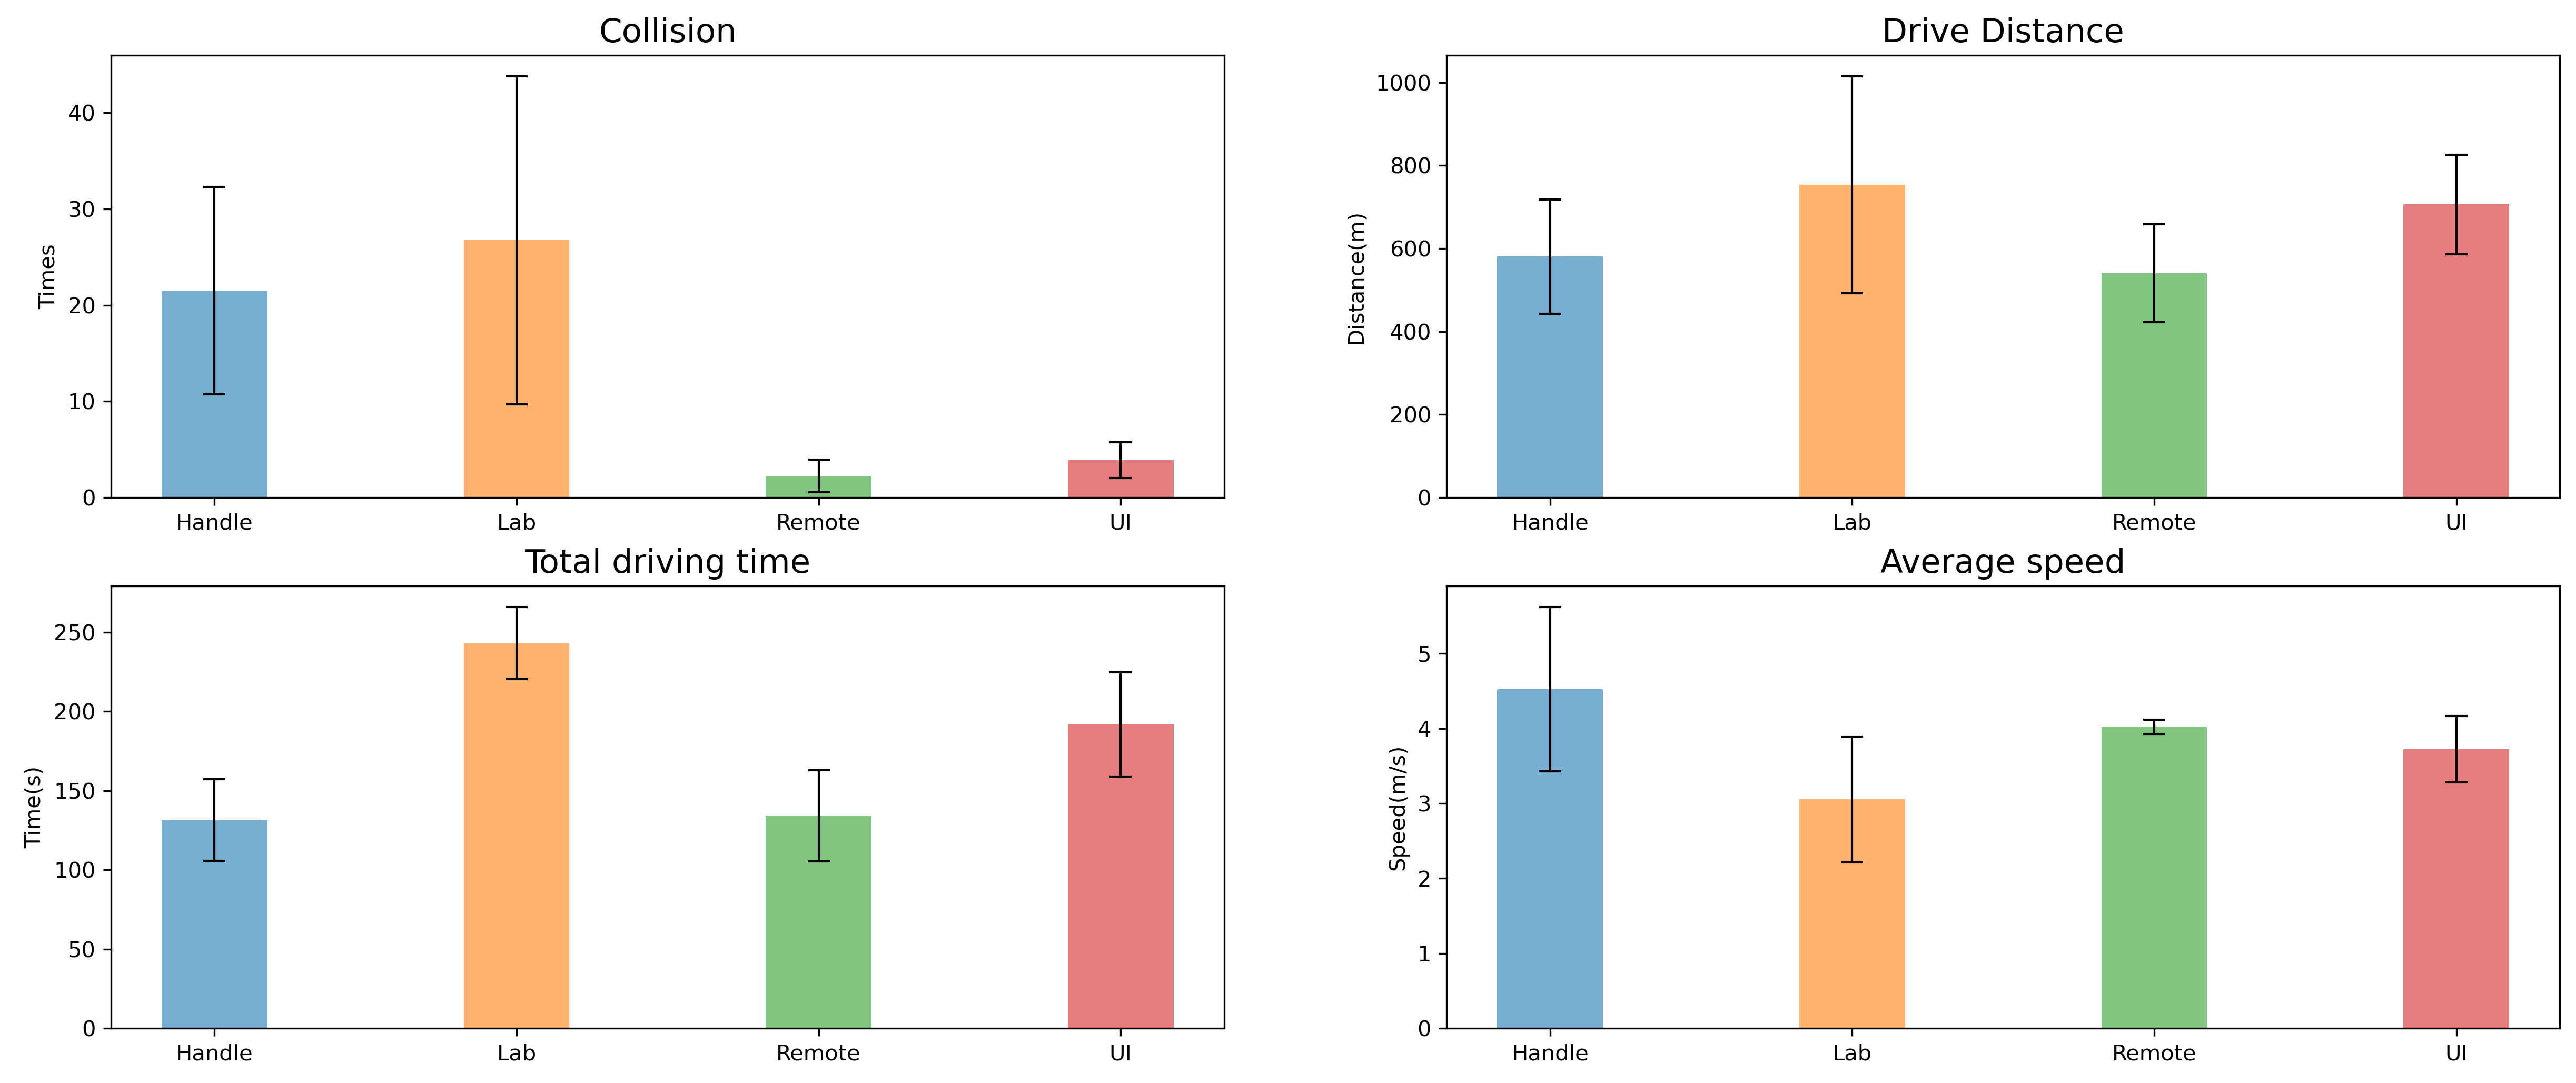
\includegraphics[width=\textwidth]{graphics/Robot Performance.png}
    \caption{Robot Performance. (All error bars indicate the standard error.)} 
    \label{fig:performance}
\end{figure}



\subsection{Rescue situation}

% \begin{wrapfigure}{r}{0.4\textwidth}
% \flushright
%   \vspace{-80pt}    % 对应高度1
%   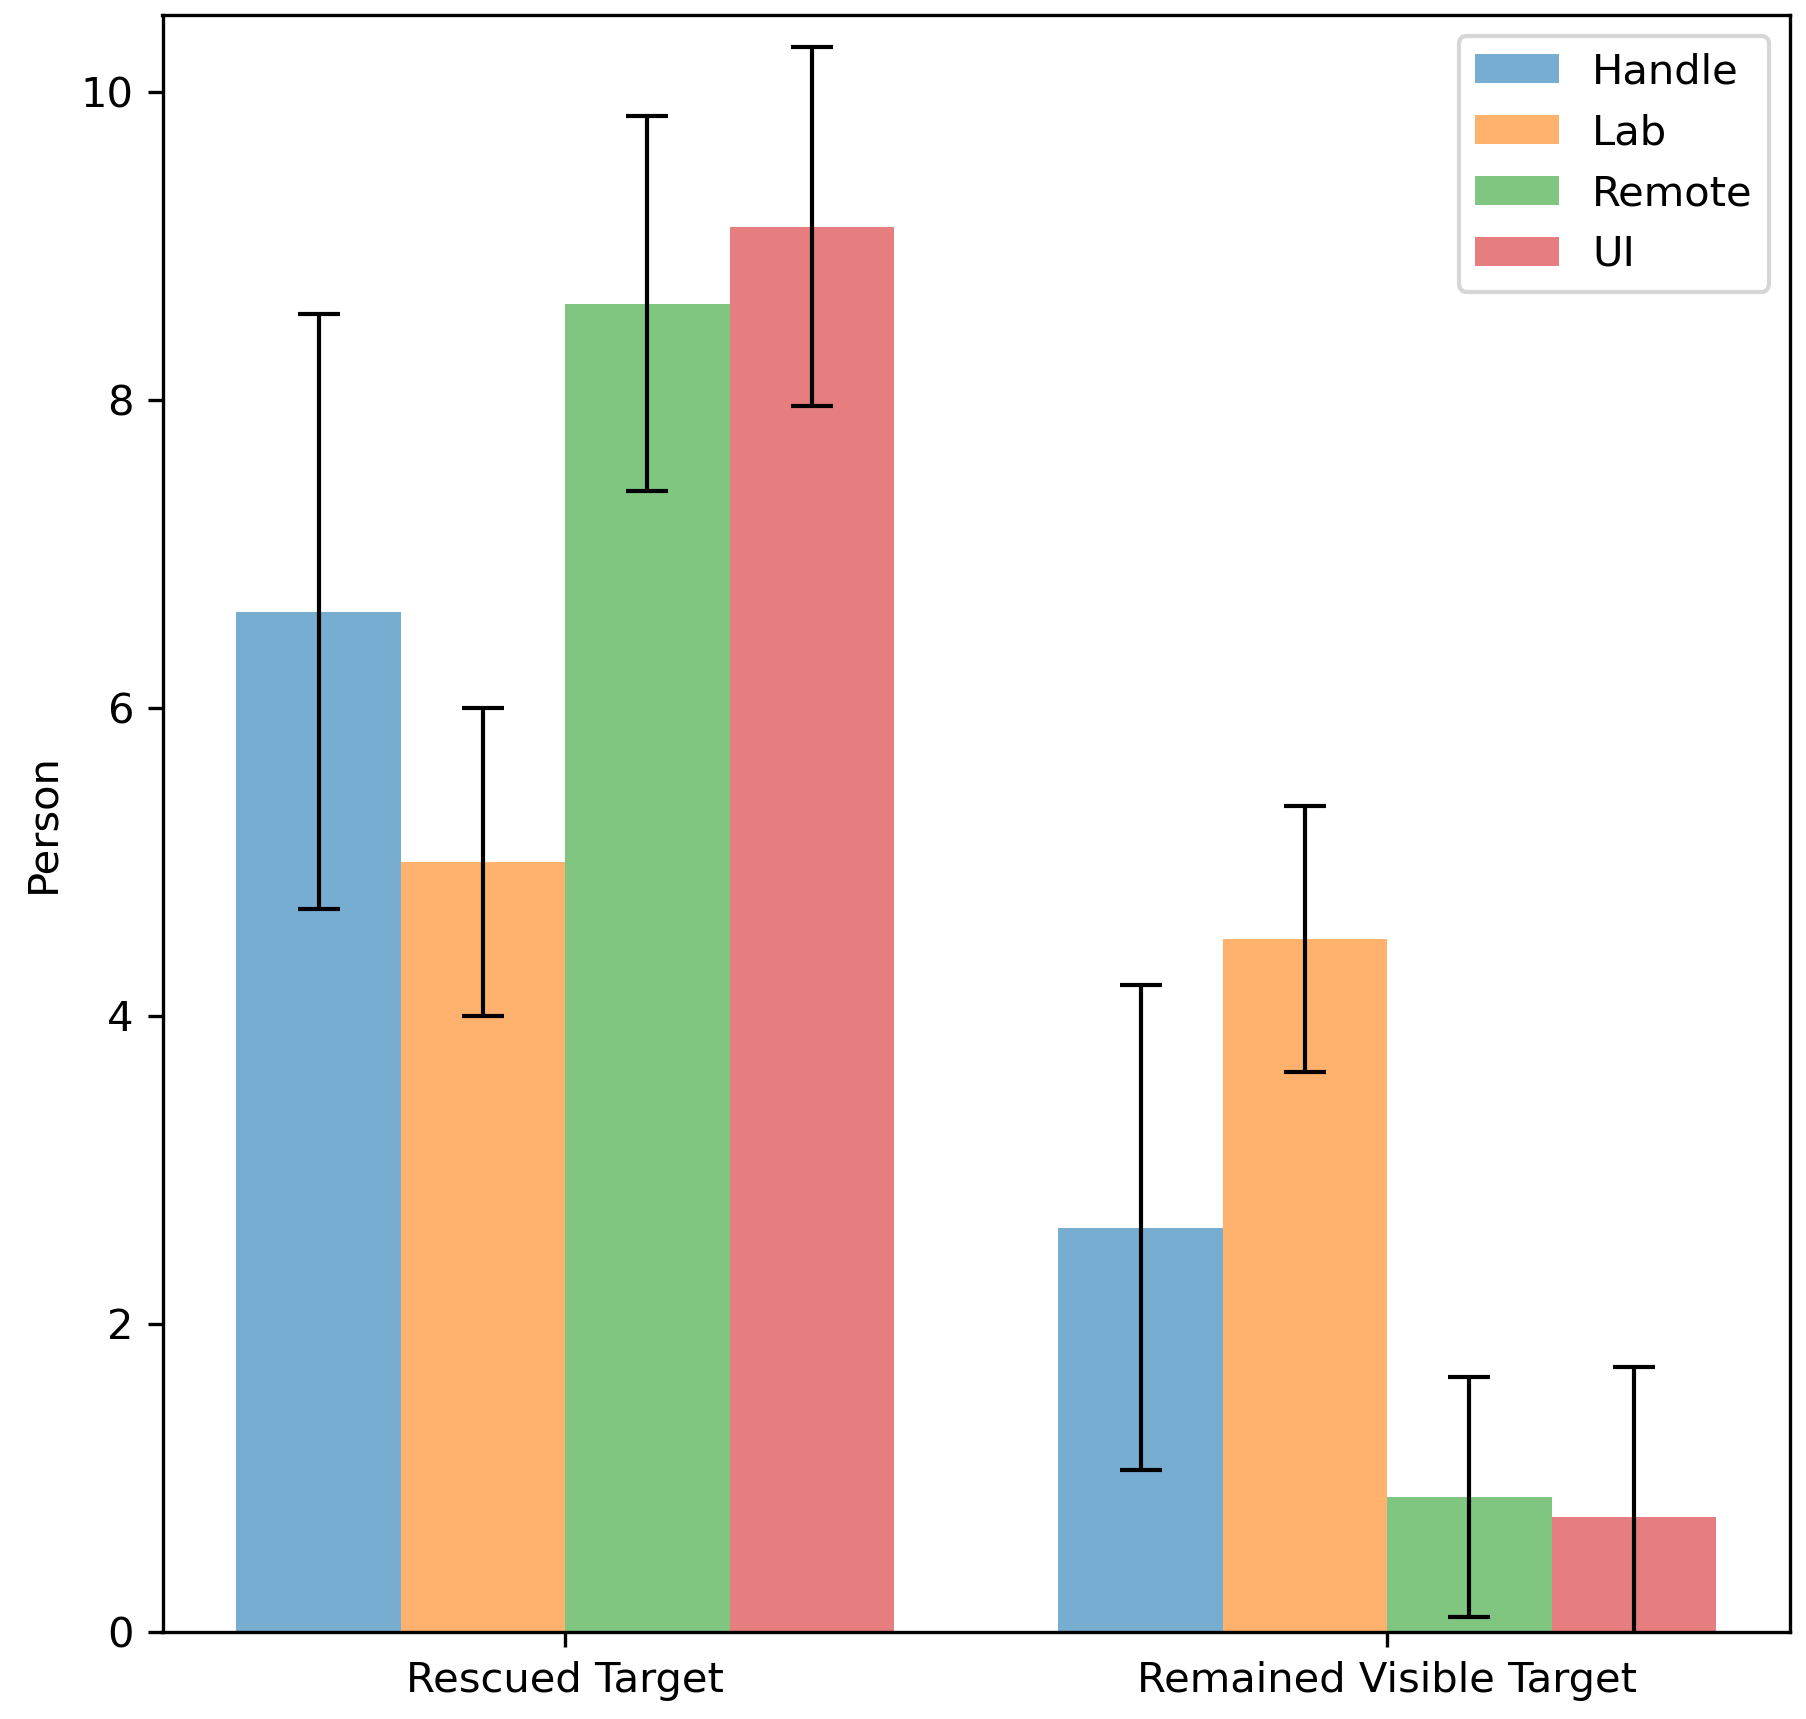
\includegraphics[height=7cm]{graphics/Rescue situation2.png}\\
%   \caption{Rescue situation. (All error bars indicate the standard error.)}
%   \label{fig:rescue}
%   \vspace{-80pt}    % 对应高度3
% \end{wrapfigure}

\begin{figure}[htbp]
    \centering
    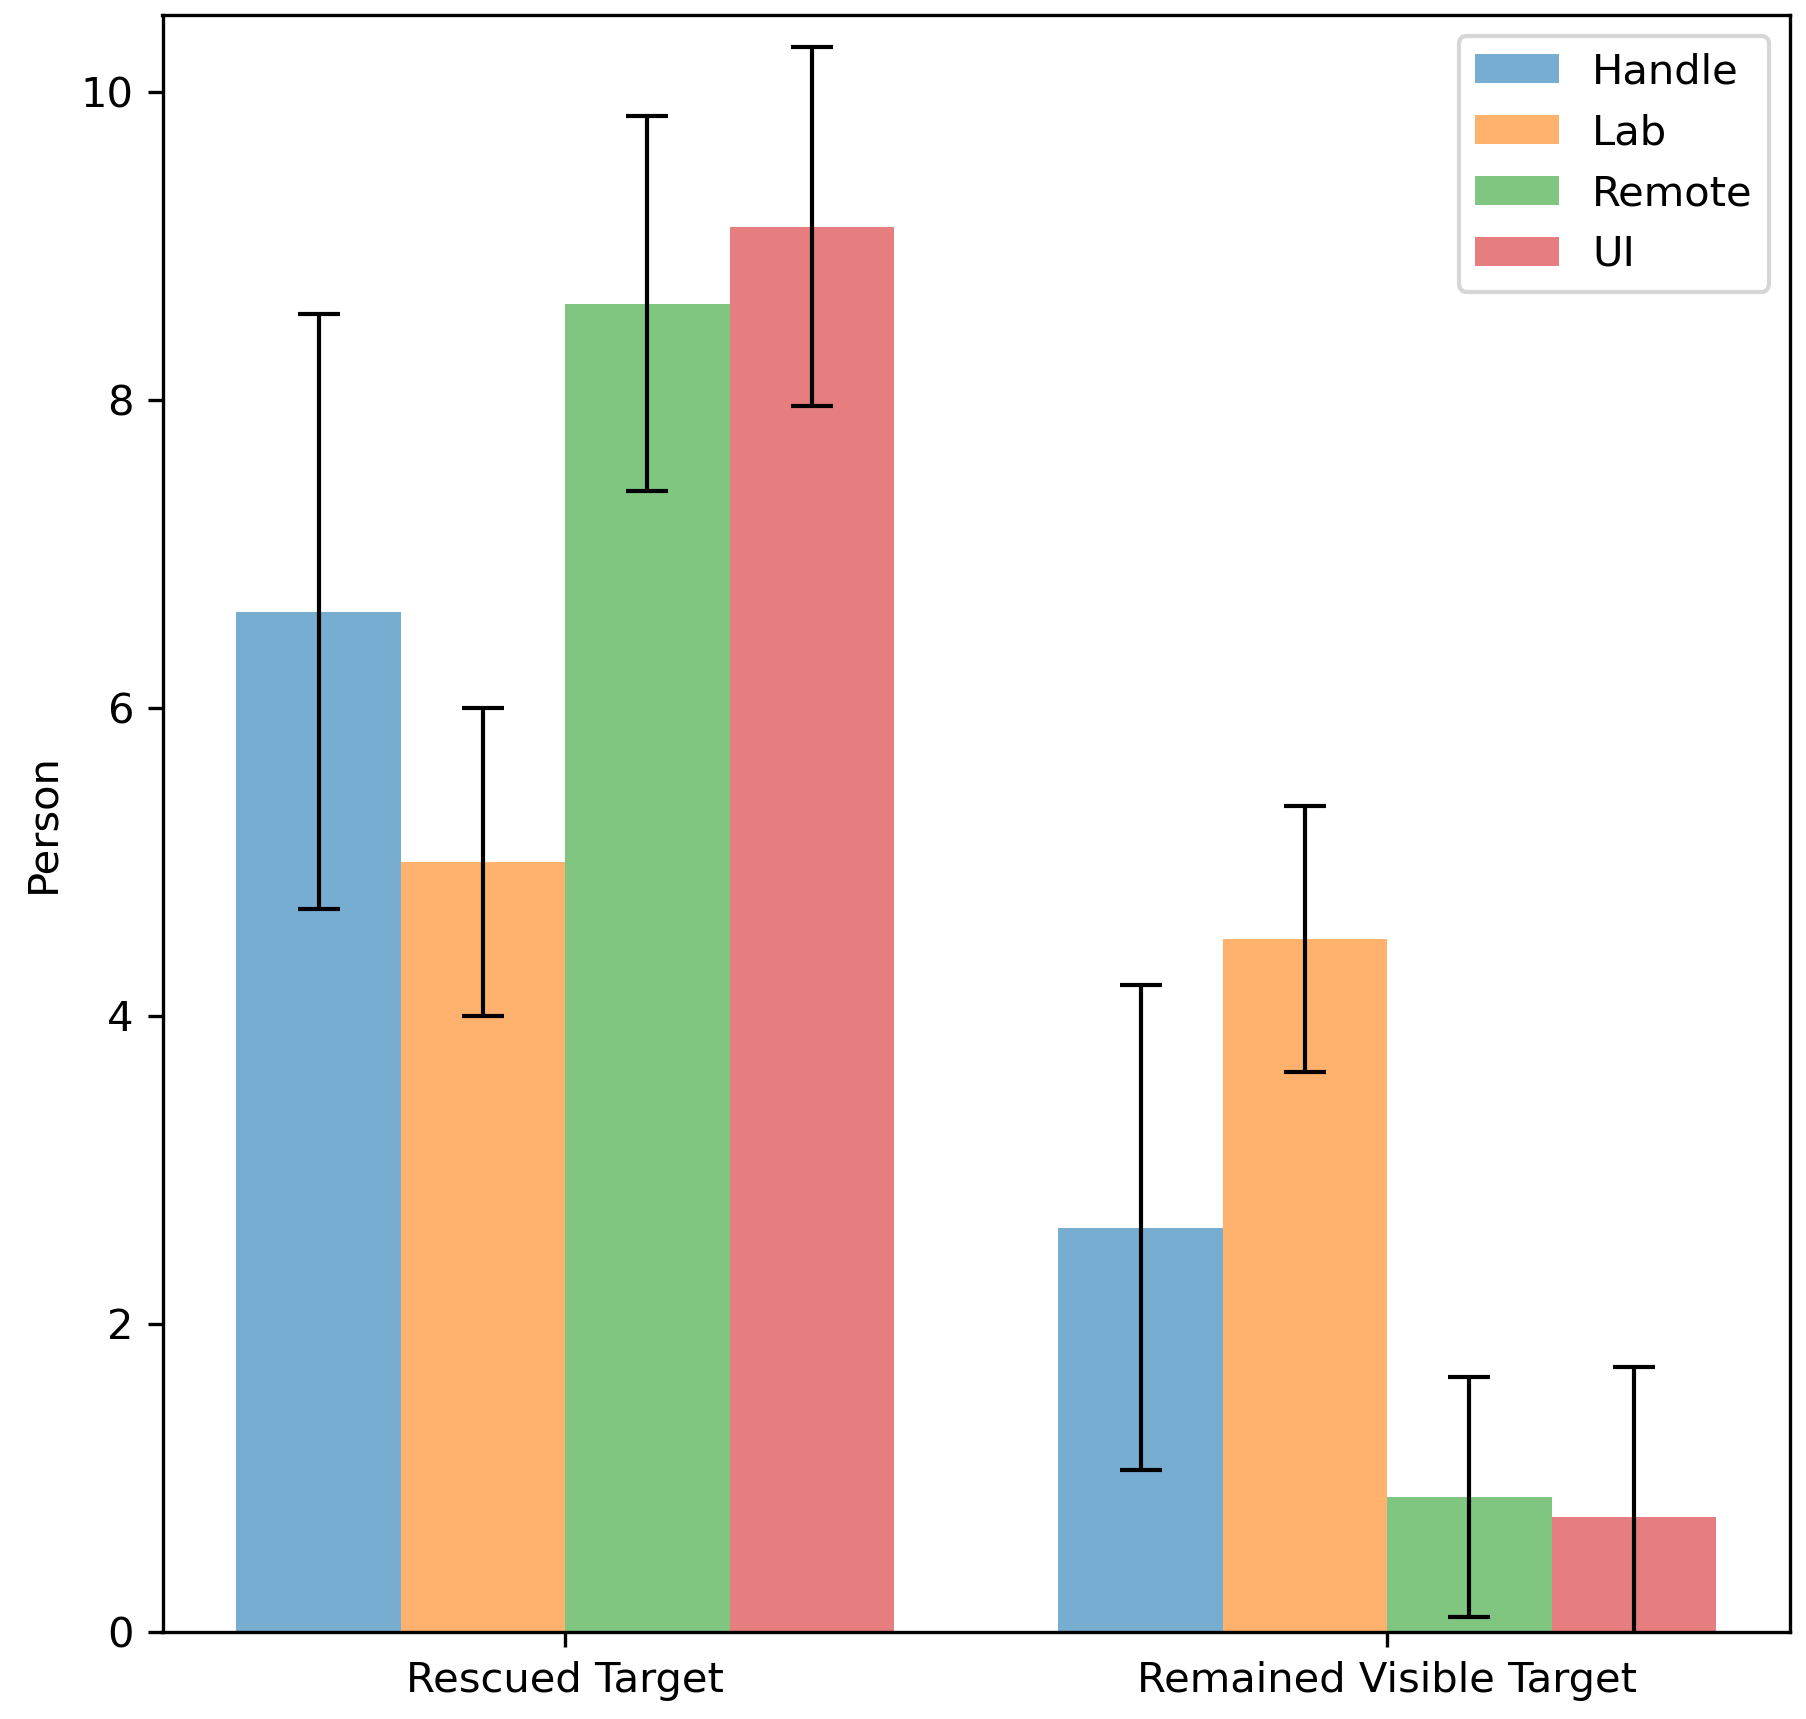
\includegraphics[height=7cm]{graphics/Rescue situation2.png}
    \caption{Rescue situation. (All error bars indicate the standard error.)} 
    \label{fig:rescue}
\end{figure}
The results of rescuing victims are shown in Figure \ref{fig:rescue}. In general, the average number of rescued victims was the highest in Remote and UI modes. In both modes, some participants rescued all the victims within the time limit, and even completed the rescue task from half a minute to one minute earlier. In the Lab Mode, the remaining visible victims were the most. This means that participants were more likely to overlook details in the scene, or even pass by the victim without noticing them. This could be attributed to the poor display quality of the screen, or it could be due to the complexity of the operation which makes the participant not have time to take into account every detail in the scene.


\subsection{TLX Score}
\begin{figure}[htbp]
    \centering
    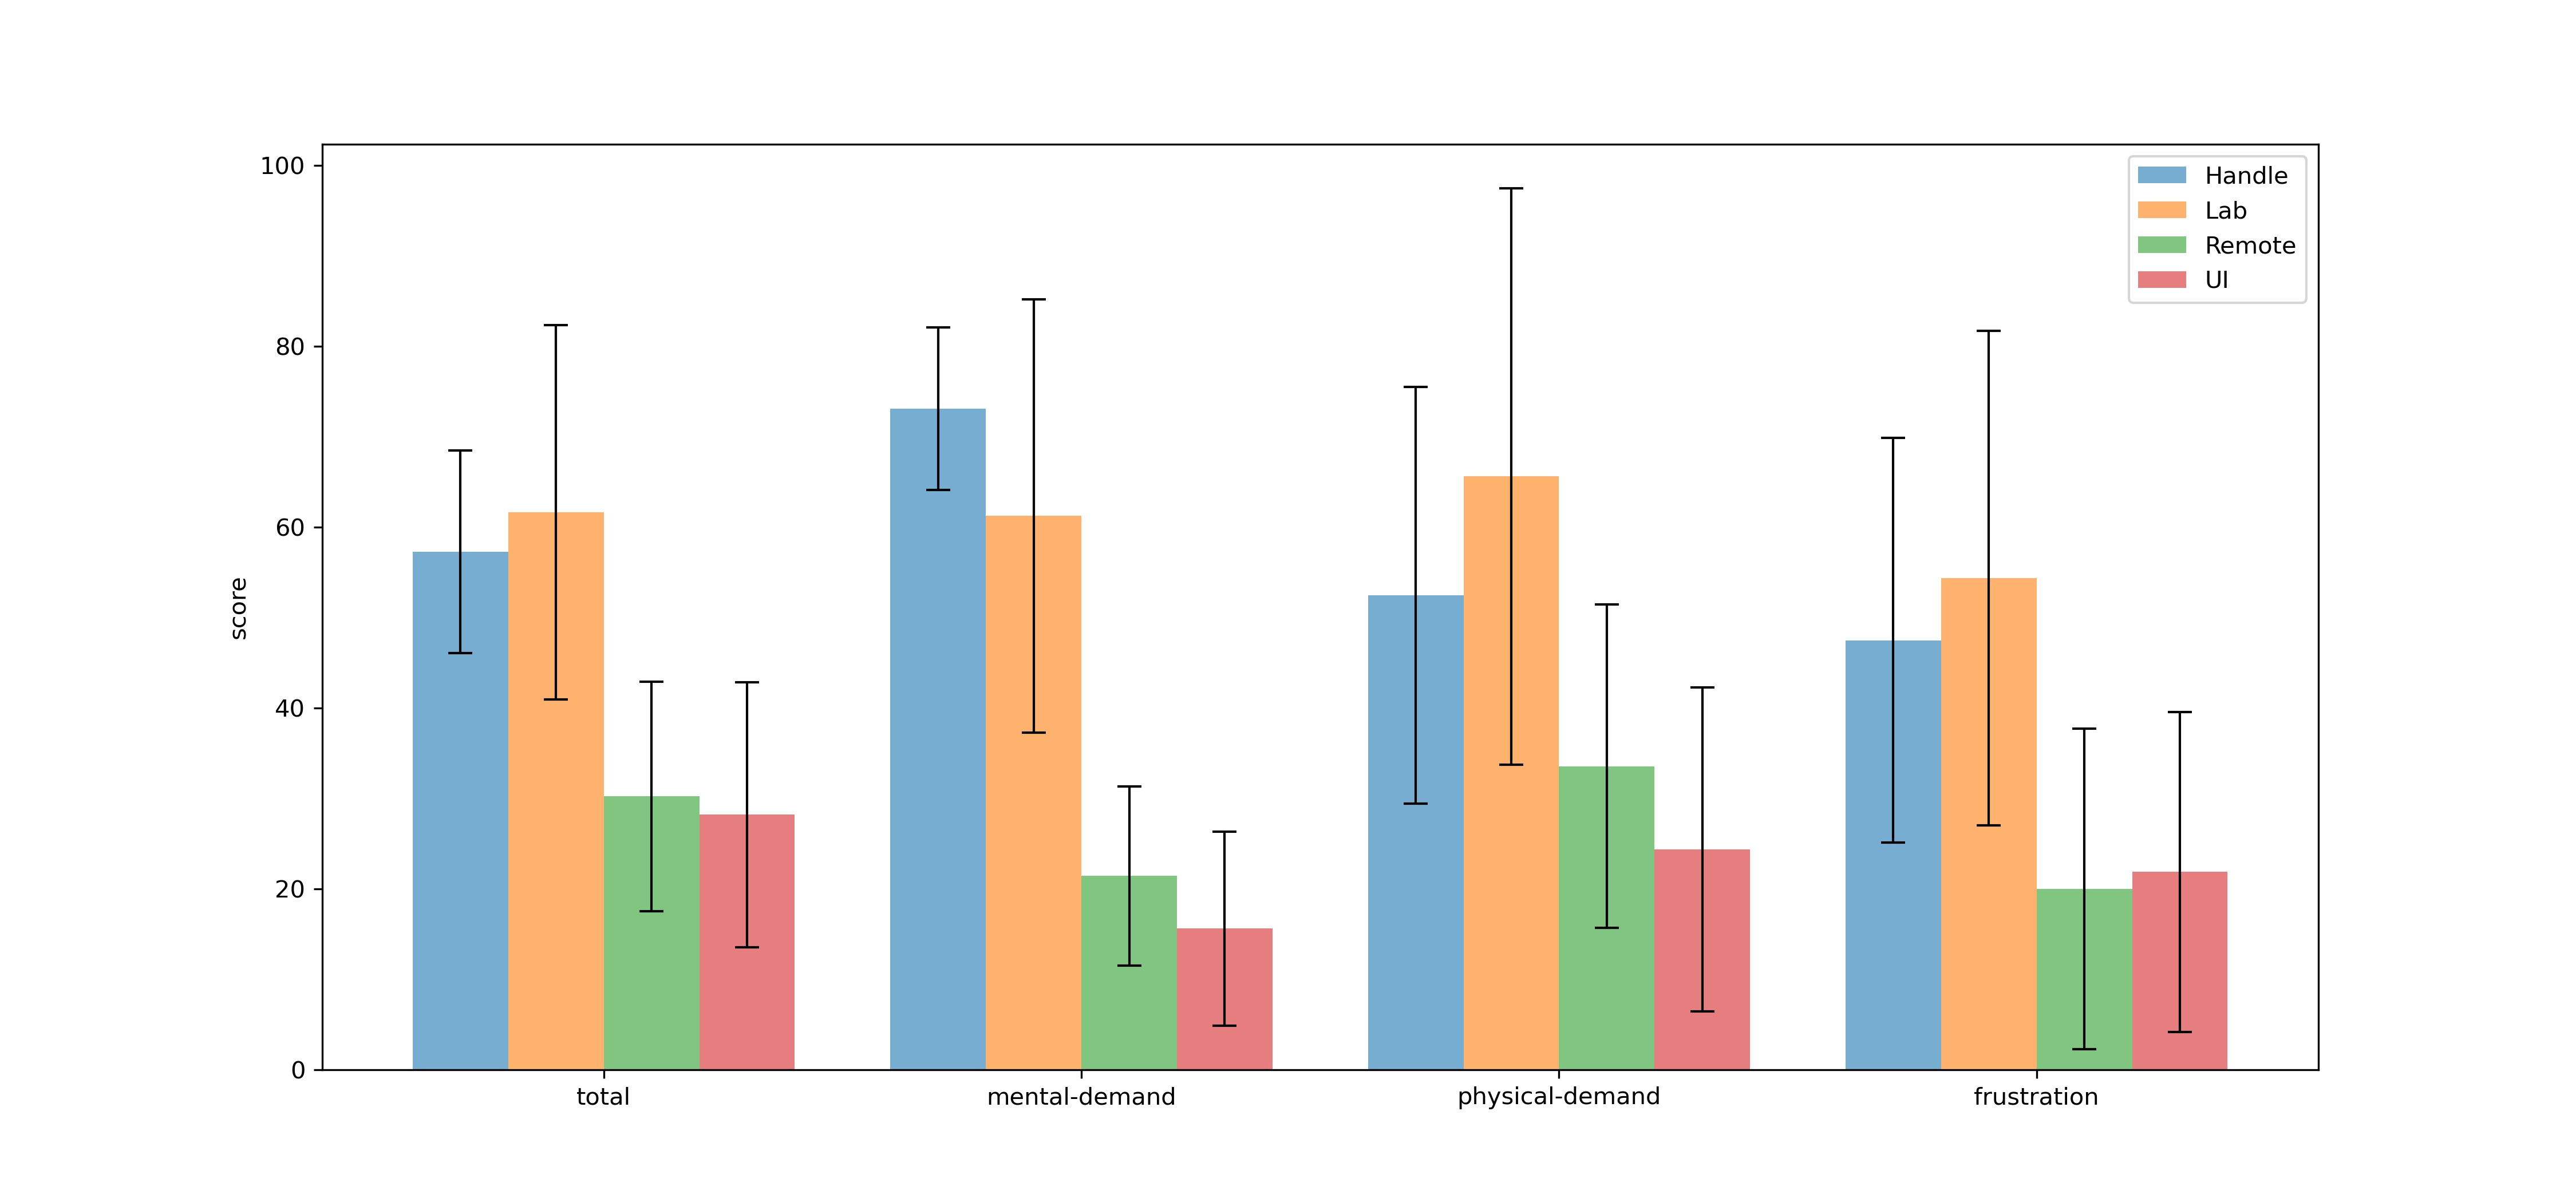
\includegraphics[width=\textwidth]{graphics/tlx6.jpg}
    \caption{The average score of \gls{tlx}. (All error bars indicate the standard error.)}
    \label{fig:tlx} 
\end{figure}
The result of \gls{tlx} reveals the perceived cognitive workload. The smaller the score is, the less workload the operation mode brings to the participant. Figure \ref{fig:tlx} contains the mean and standard error of each scale. The standard error was significant for each scale because participants could only evaluate the workload of each mode of operation relatively, and they had different standard values in mind. 

In this subsection, the total score will be analyzed. Three of the subjective subscales are selected additionally for detailed explanation.

As can be seen, similar score could be found for each scale in Lab Mode and Handle Mode, and their values were significantly worse than the other two modes. In the majority of cases, the average load in these two modes was almost twice as high as in Remote and UI modes. ($total_{Handle} = 57.29$, $total_{Lab} = 61.67$, $total_{Remote} = 30.24$, $total_{UI} = 28.23$) 

The difference in scores was huge in terms of mental demand. ($mental_{Handle} = 73.125$, $mental_{Lab} = 61.25$, $mental_{Remote} = 21.43$, $mental_{UI} = 15.63$) The Handle Mode required the most mental activity. Participants said they needed to recall what buttons to press to achieve a certain effect or consider how to turn the robot to get it moving towards the desired position. They also had to pay attention to the distance between themselves and the robots so that the robots would not leave their sight.

 Physical demand in Lab Mode was highest. It was observed that they frequently looked up and down to view different screens. In addition, some participants maintained their arms in a flat position while operating the virtual joystick, which also caused some fatigue on the arms. 

In Lab Mode and Handle Mode, they felt more negative emotions, such as irritability, stress, etc. ($frustration_{Handle} = 47.5$, $frustration_{Lab} = 54.38$, $frustration_{Remote} = 20$, $frustration_{UI} = 21.88$.)

Overall, the Remote and UI modes received better scores on \gls{tlx}.


% \begin{figure}[htbp]
%     \centering
%     \subfigure{
%         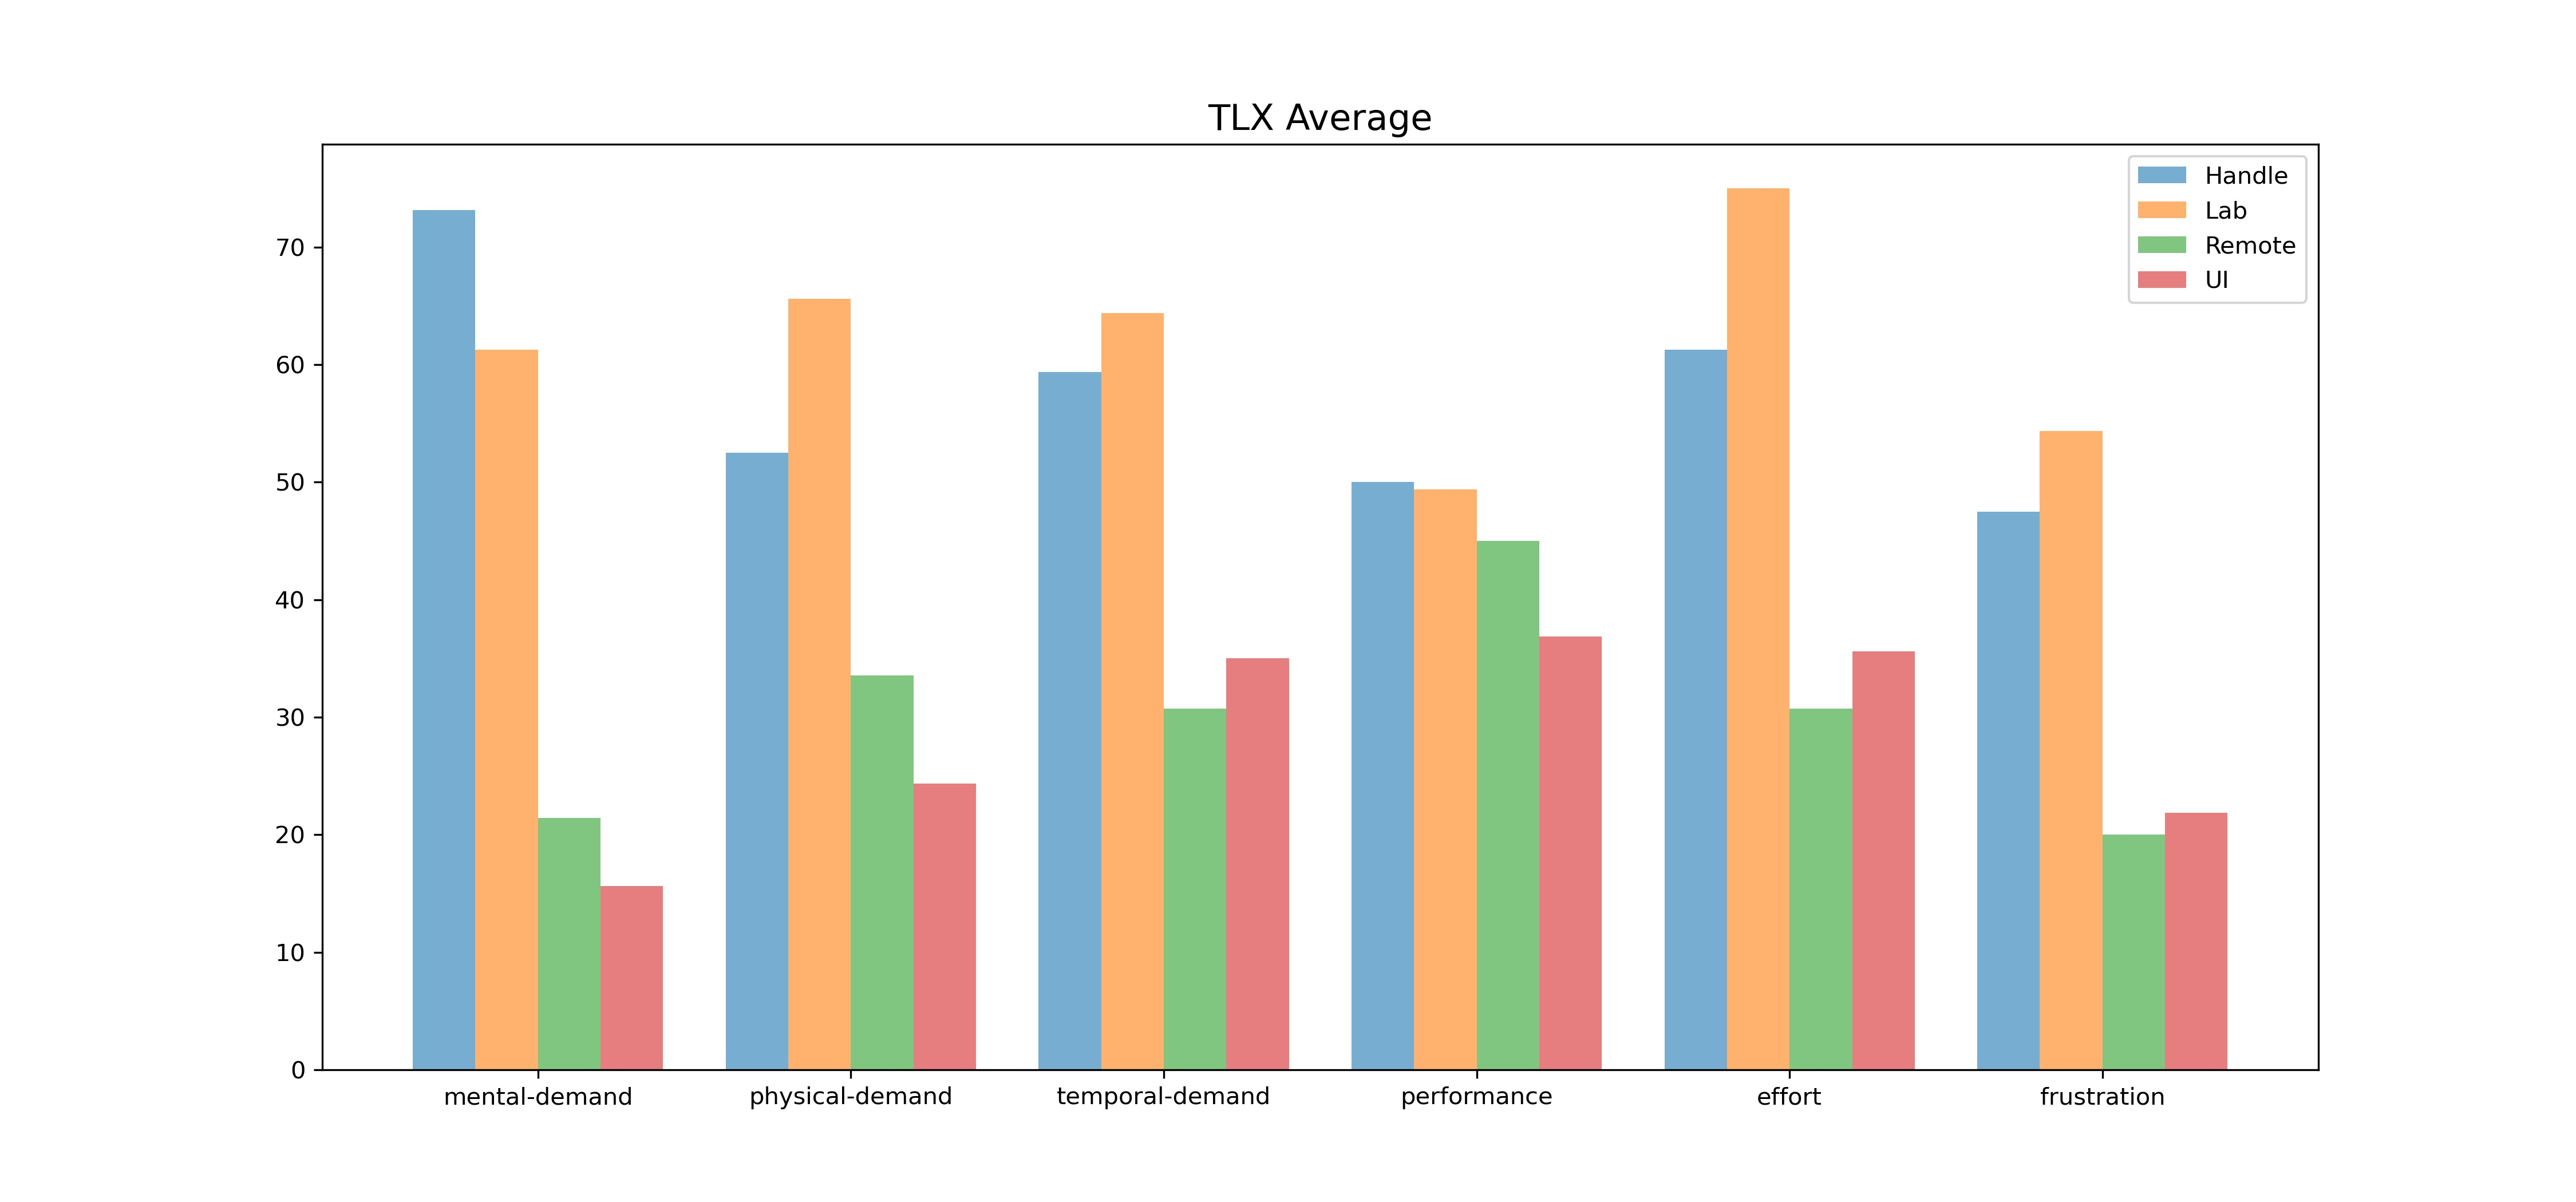
\includegraphics[width=\textwidth]{graphics/summary.jpg}
%     }
%     \subfigure{ 
%         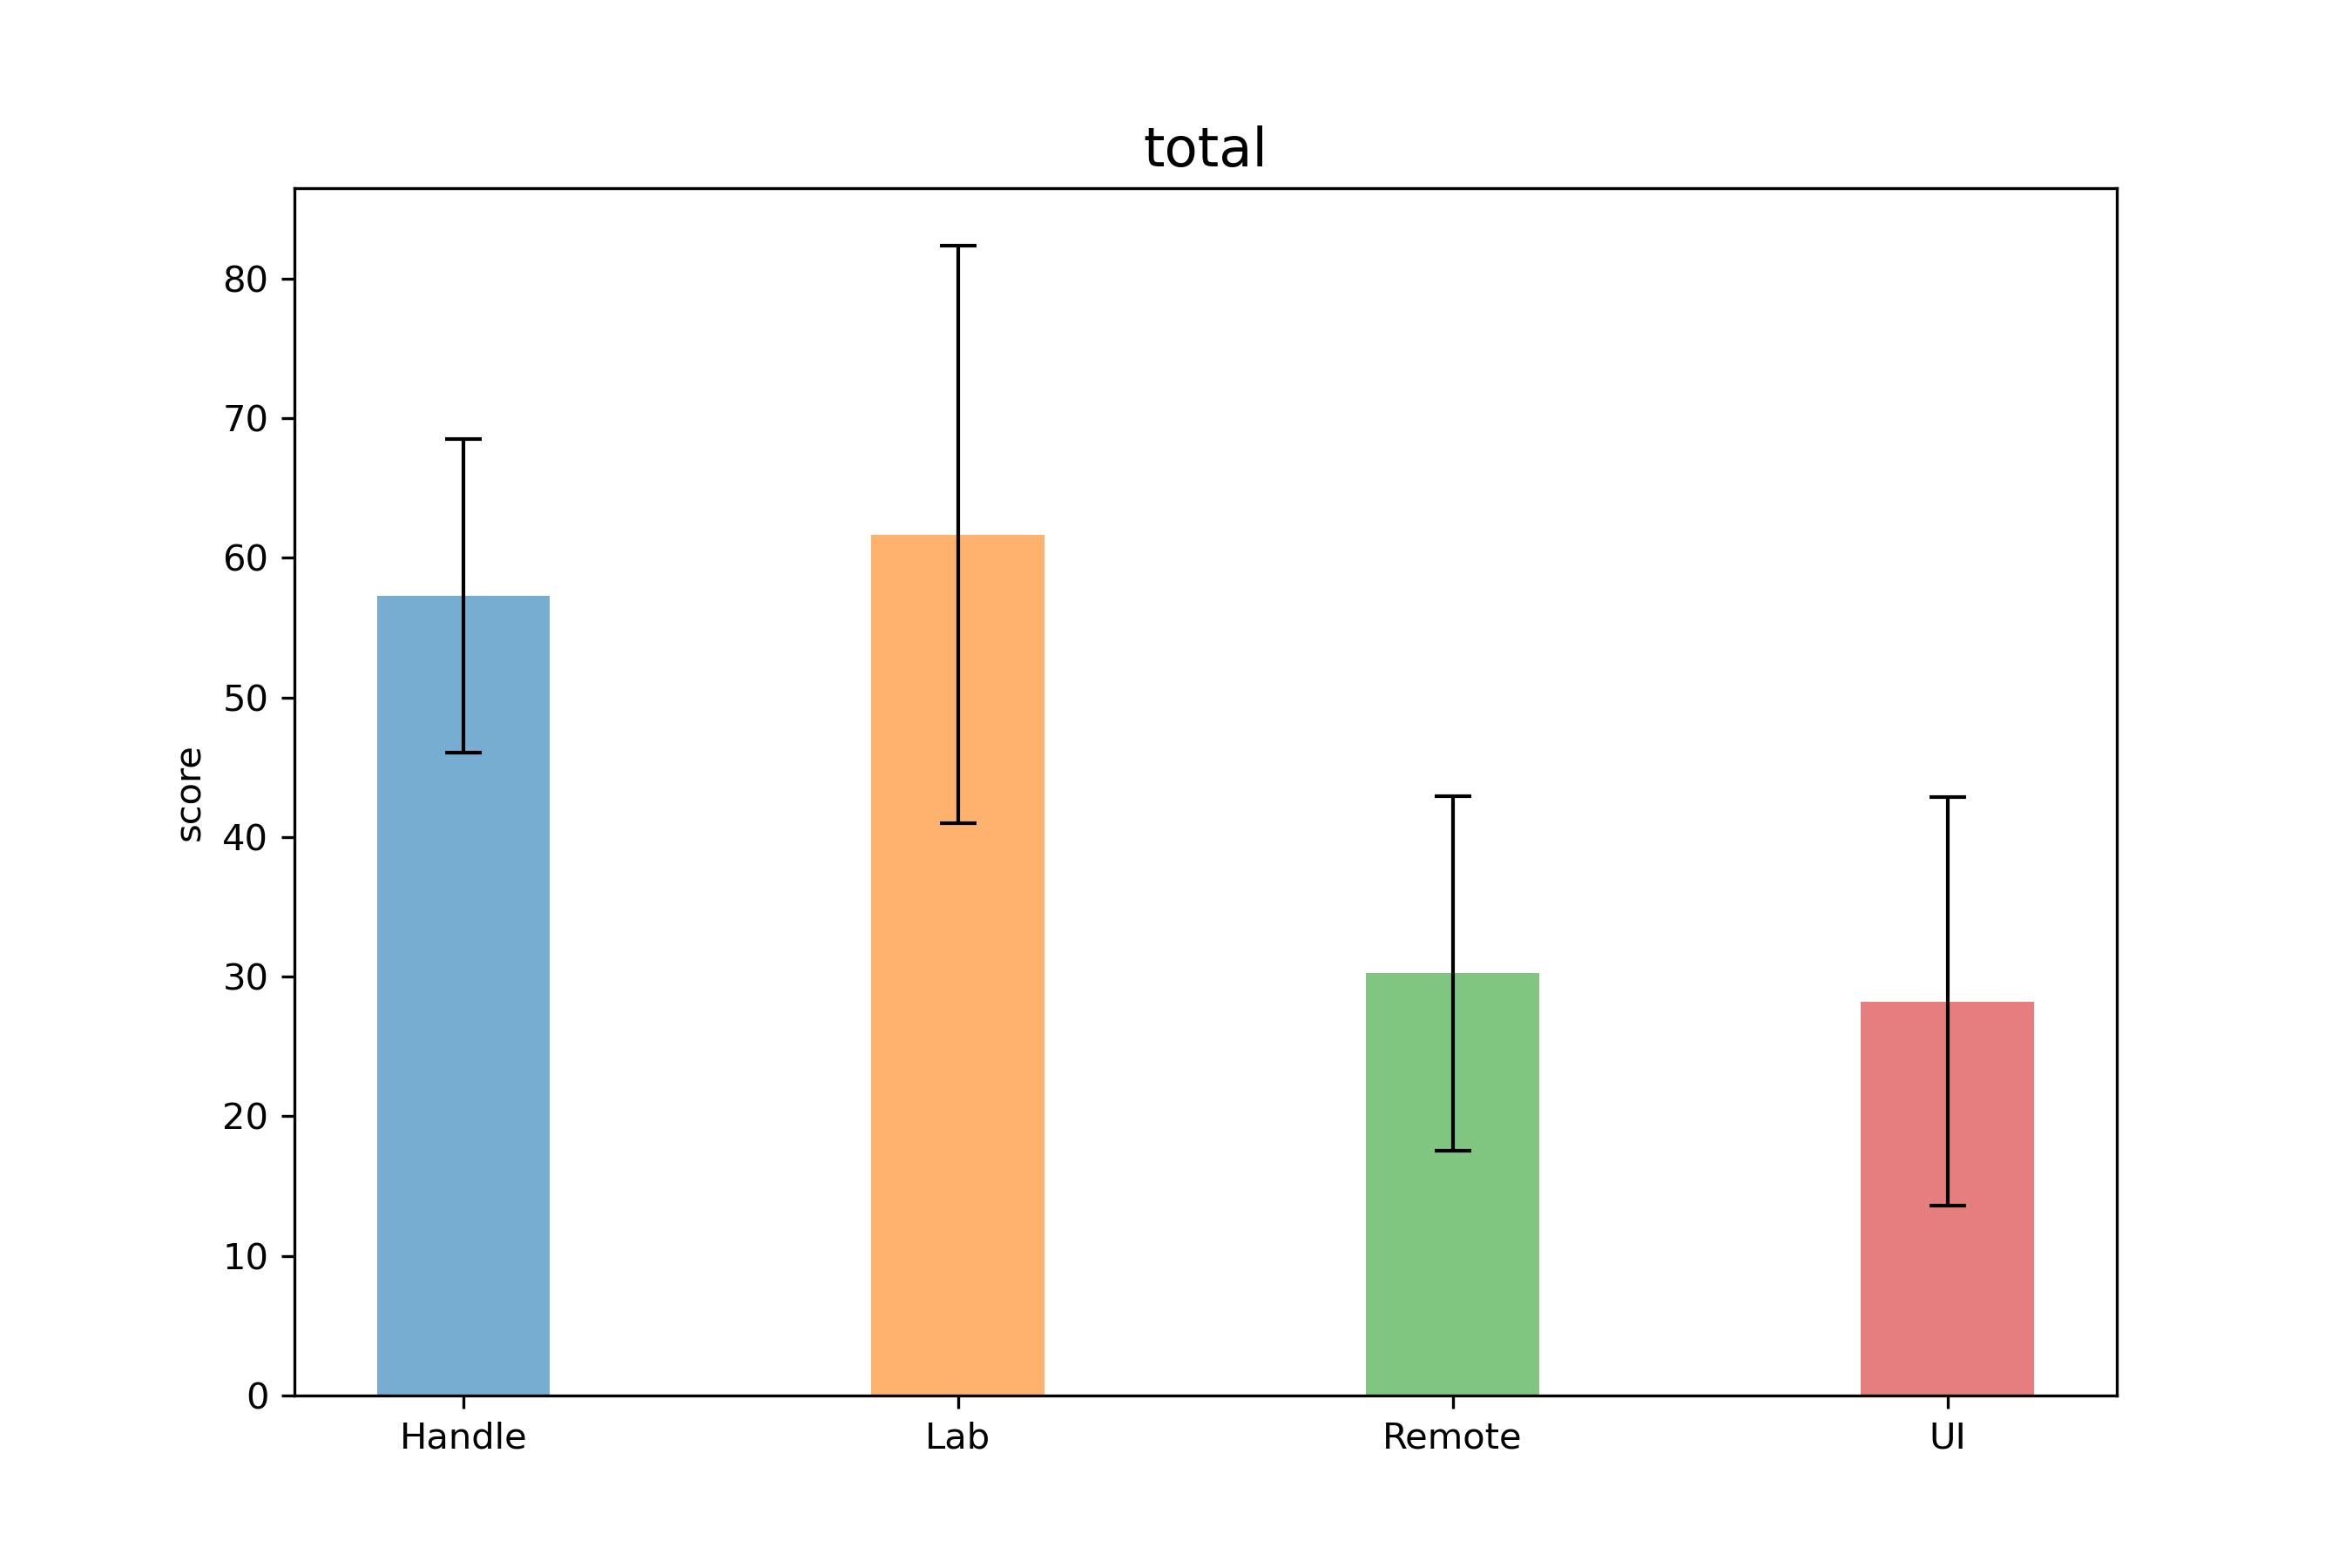
\includegraphics[width=\textwidth]{graphics/total.png}
%     }
%     \caption{TLX Score.expain...}
%     \label{fig:tlx} 
% \end{figure}



\subsection{Likert Questionnaire Results}
After each test was completed, participants were also asked to fill out a questionnaire. The results can be seen in Figure \ref{fig:liker}. The questionnaire uses a 5-point Likert scale. 1 means that participants considered that their situations did not fit the question description at all. 5 indicates that their situations fit perfectly.
\begin{figure}[htbp]
    \centering
    \subfigure{
        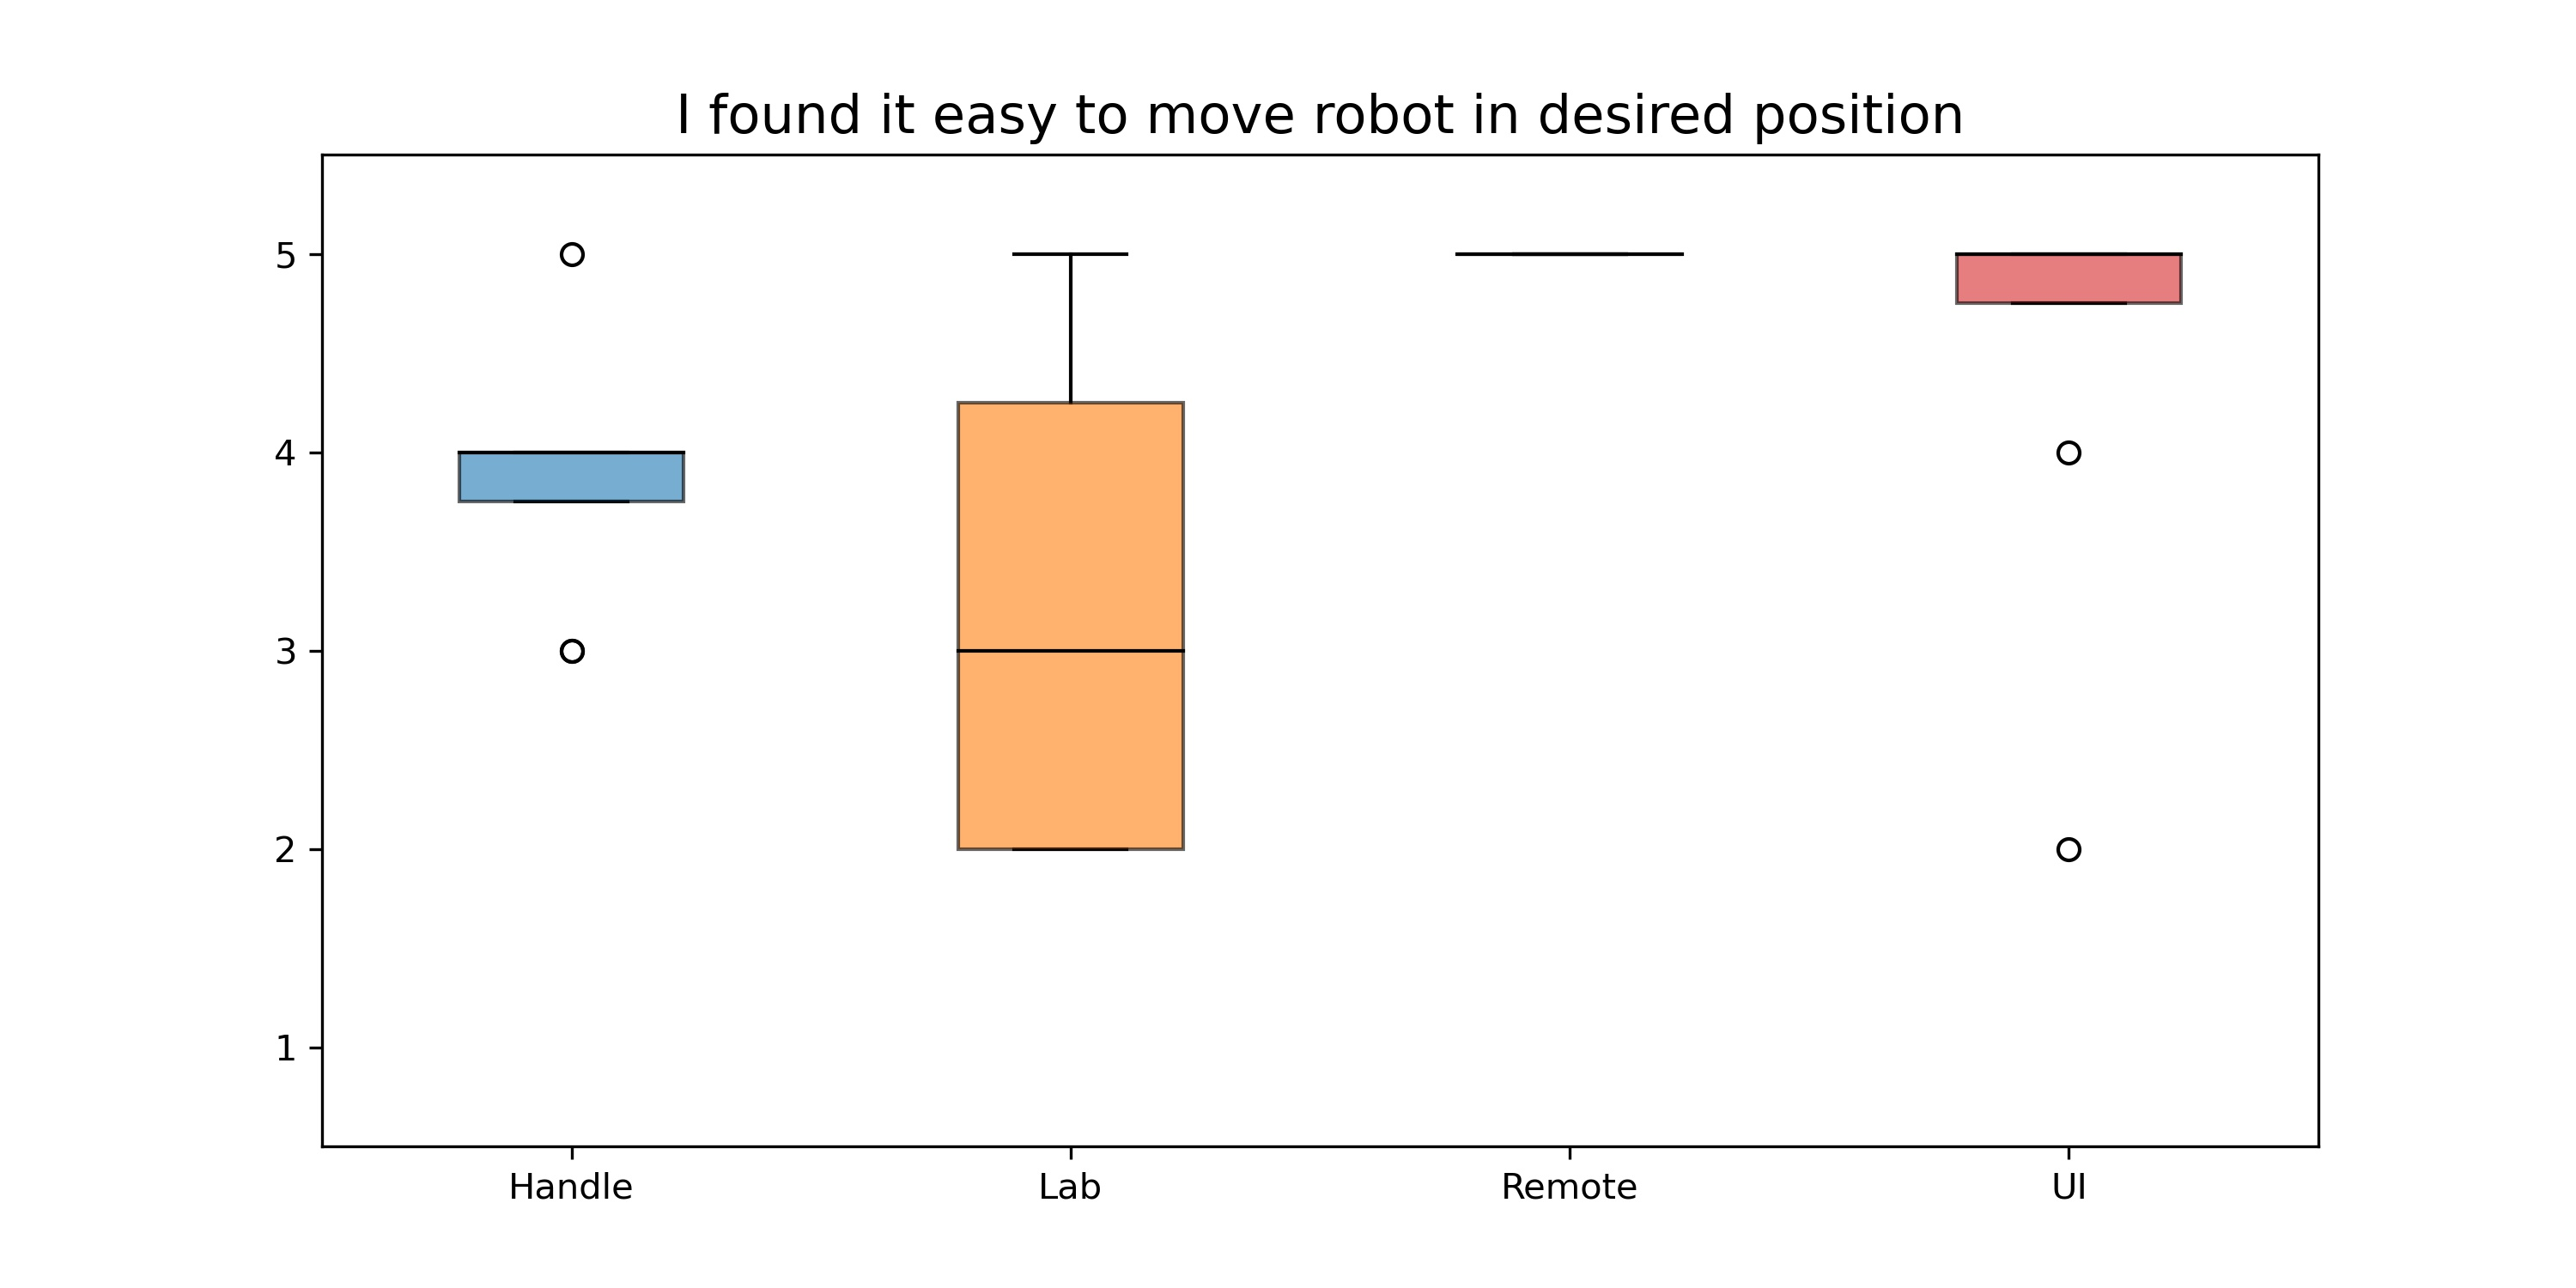
\includegraphics[height=7cm]{graphics/I found it easy to move robot in desired position.jpg}
    }
    \subfigure{ 
        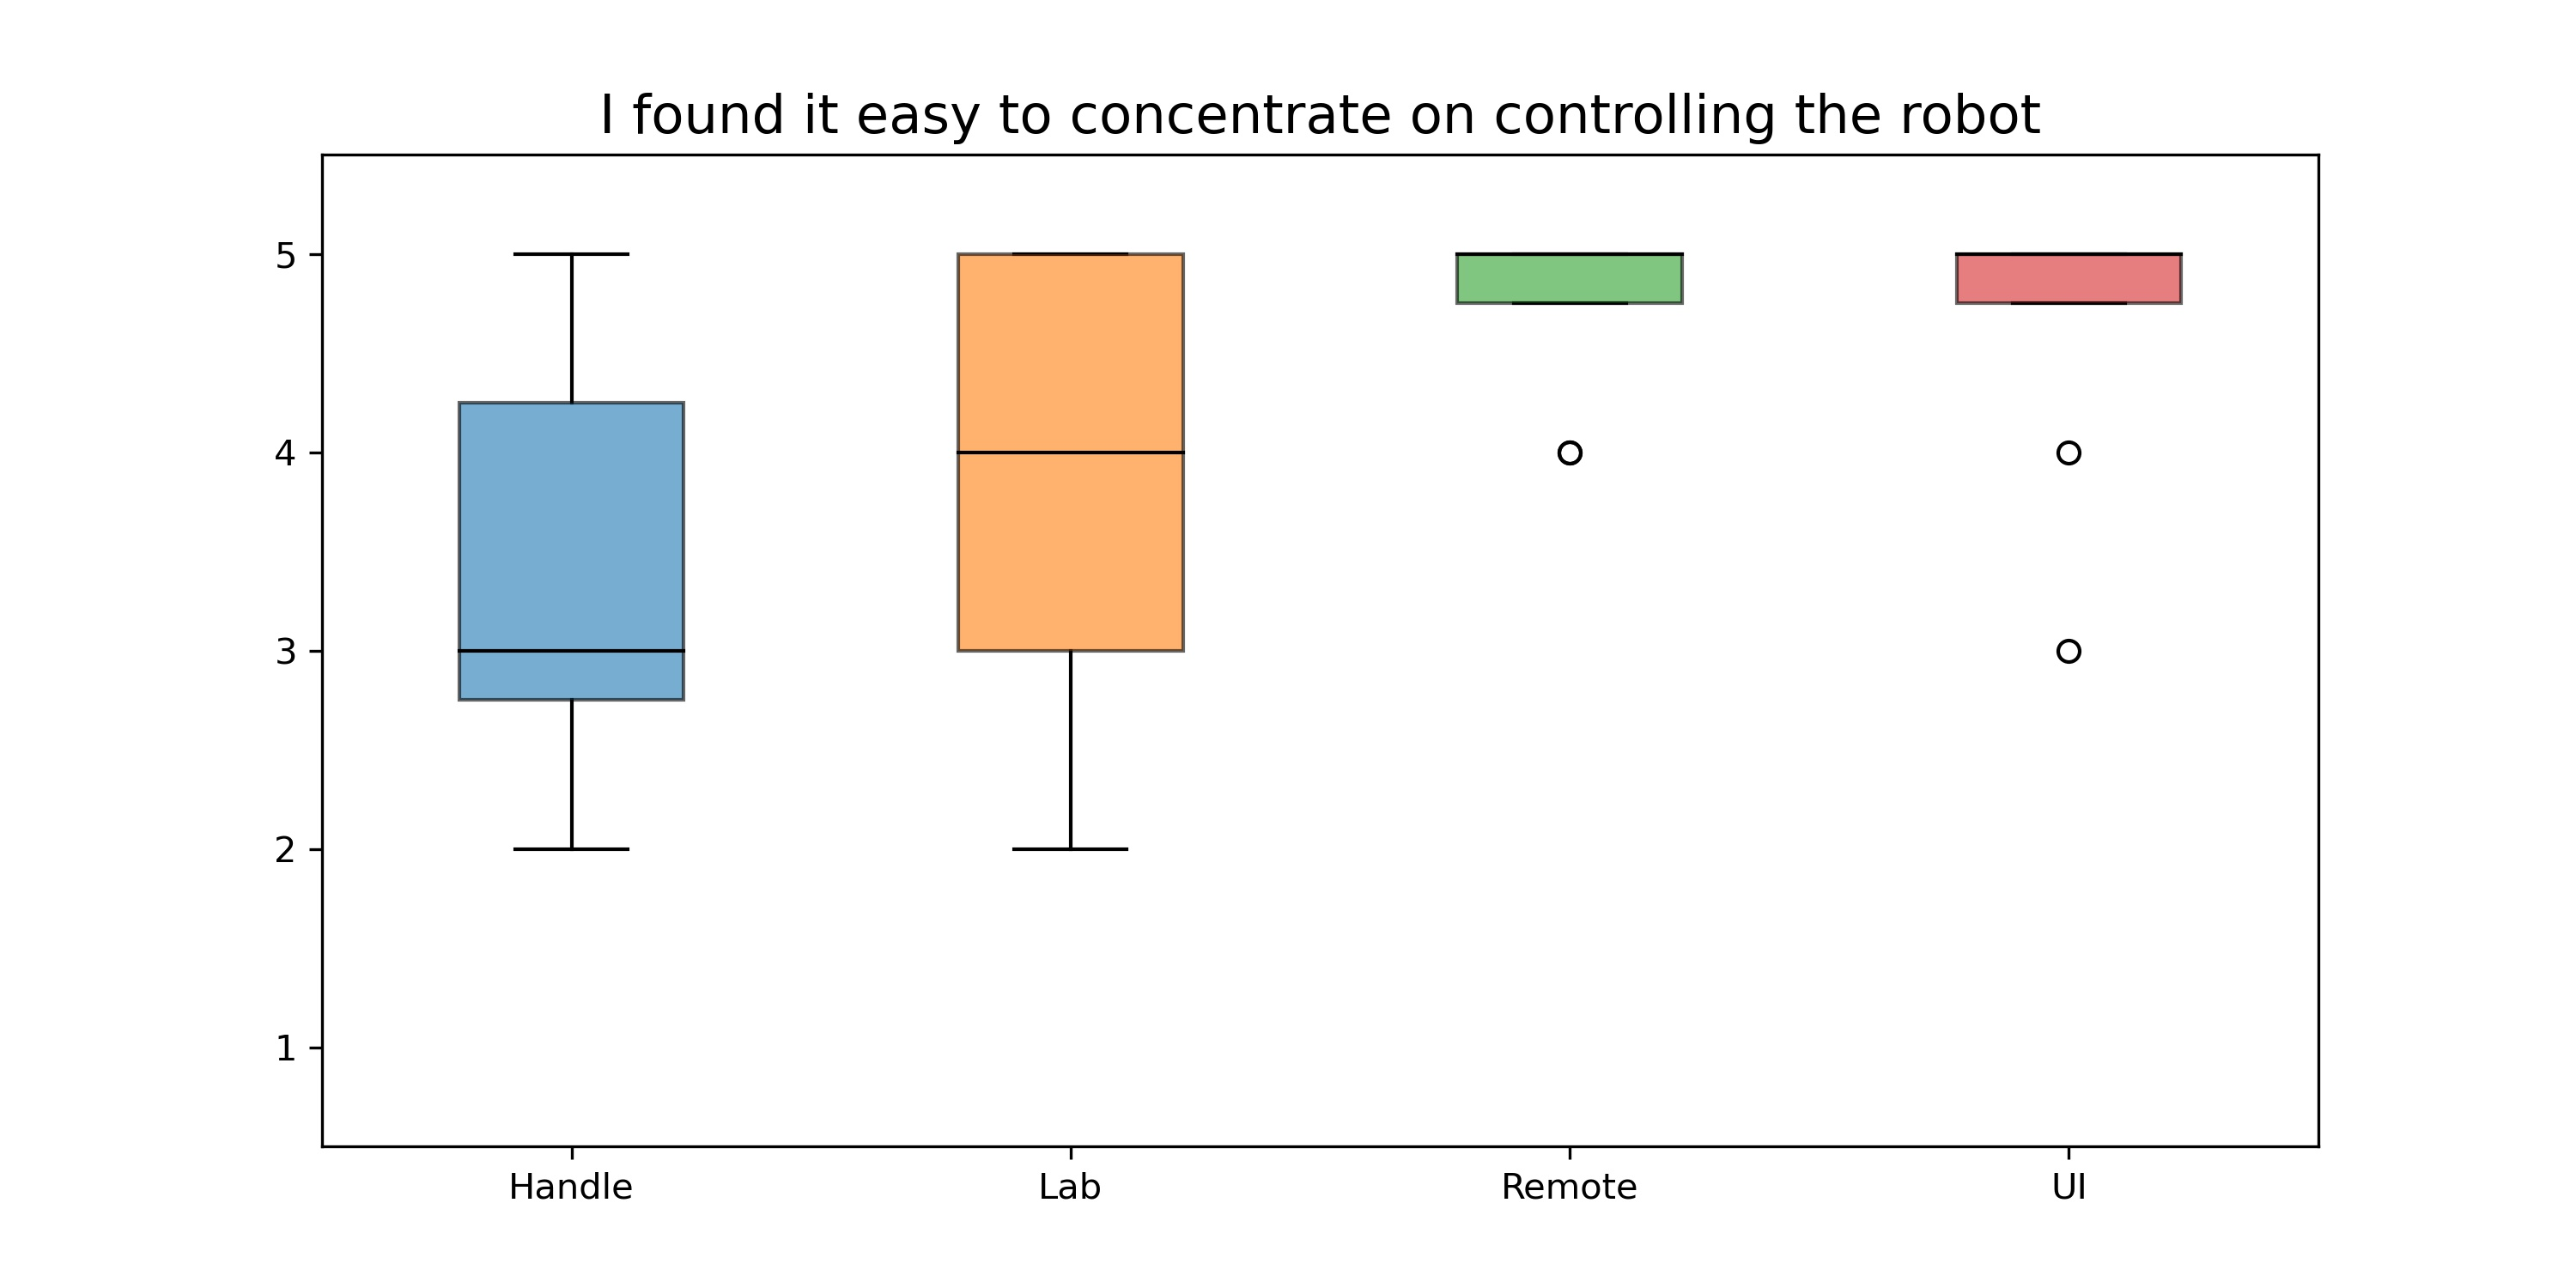
\includegraphics[height=7cm]{graphics/I found it easy to concentrate on controlling the robot.jpg}
    }
    \subfigure{ 
        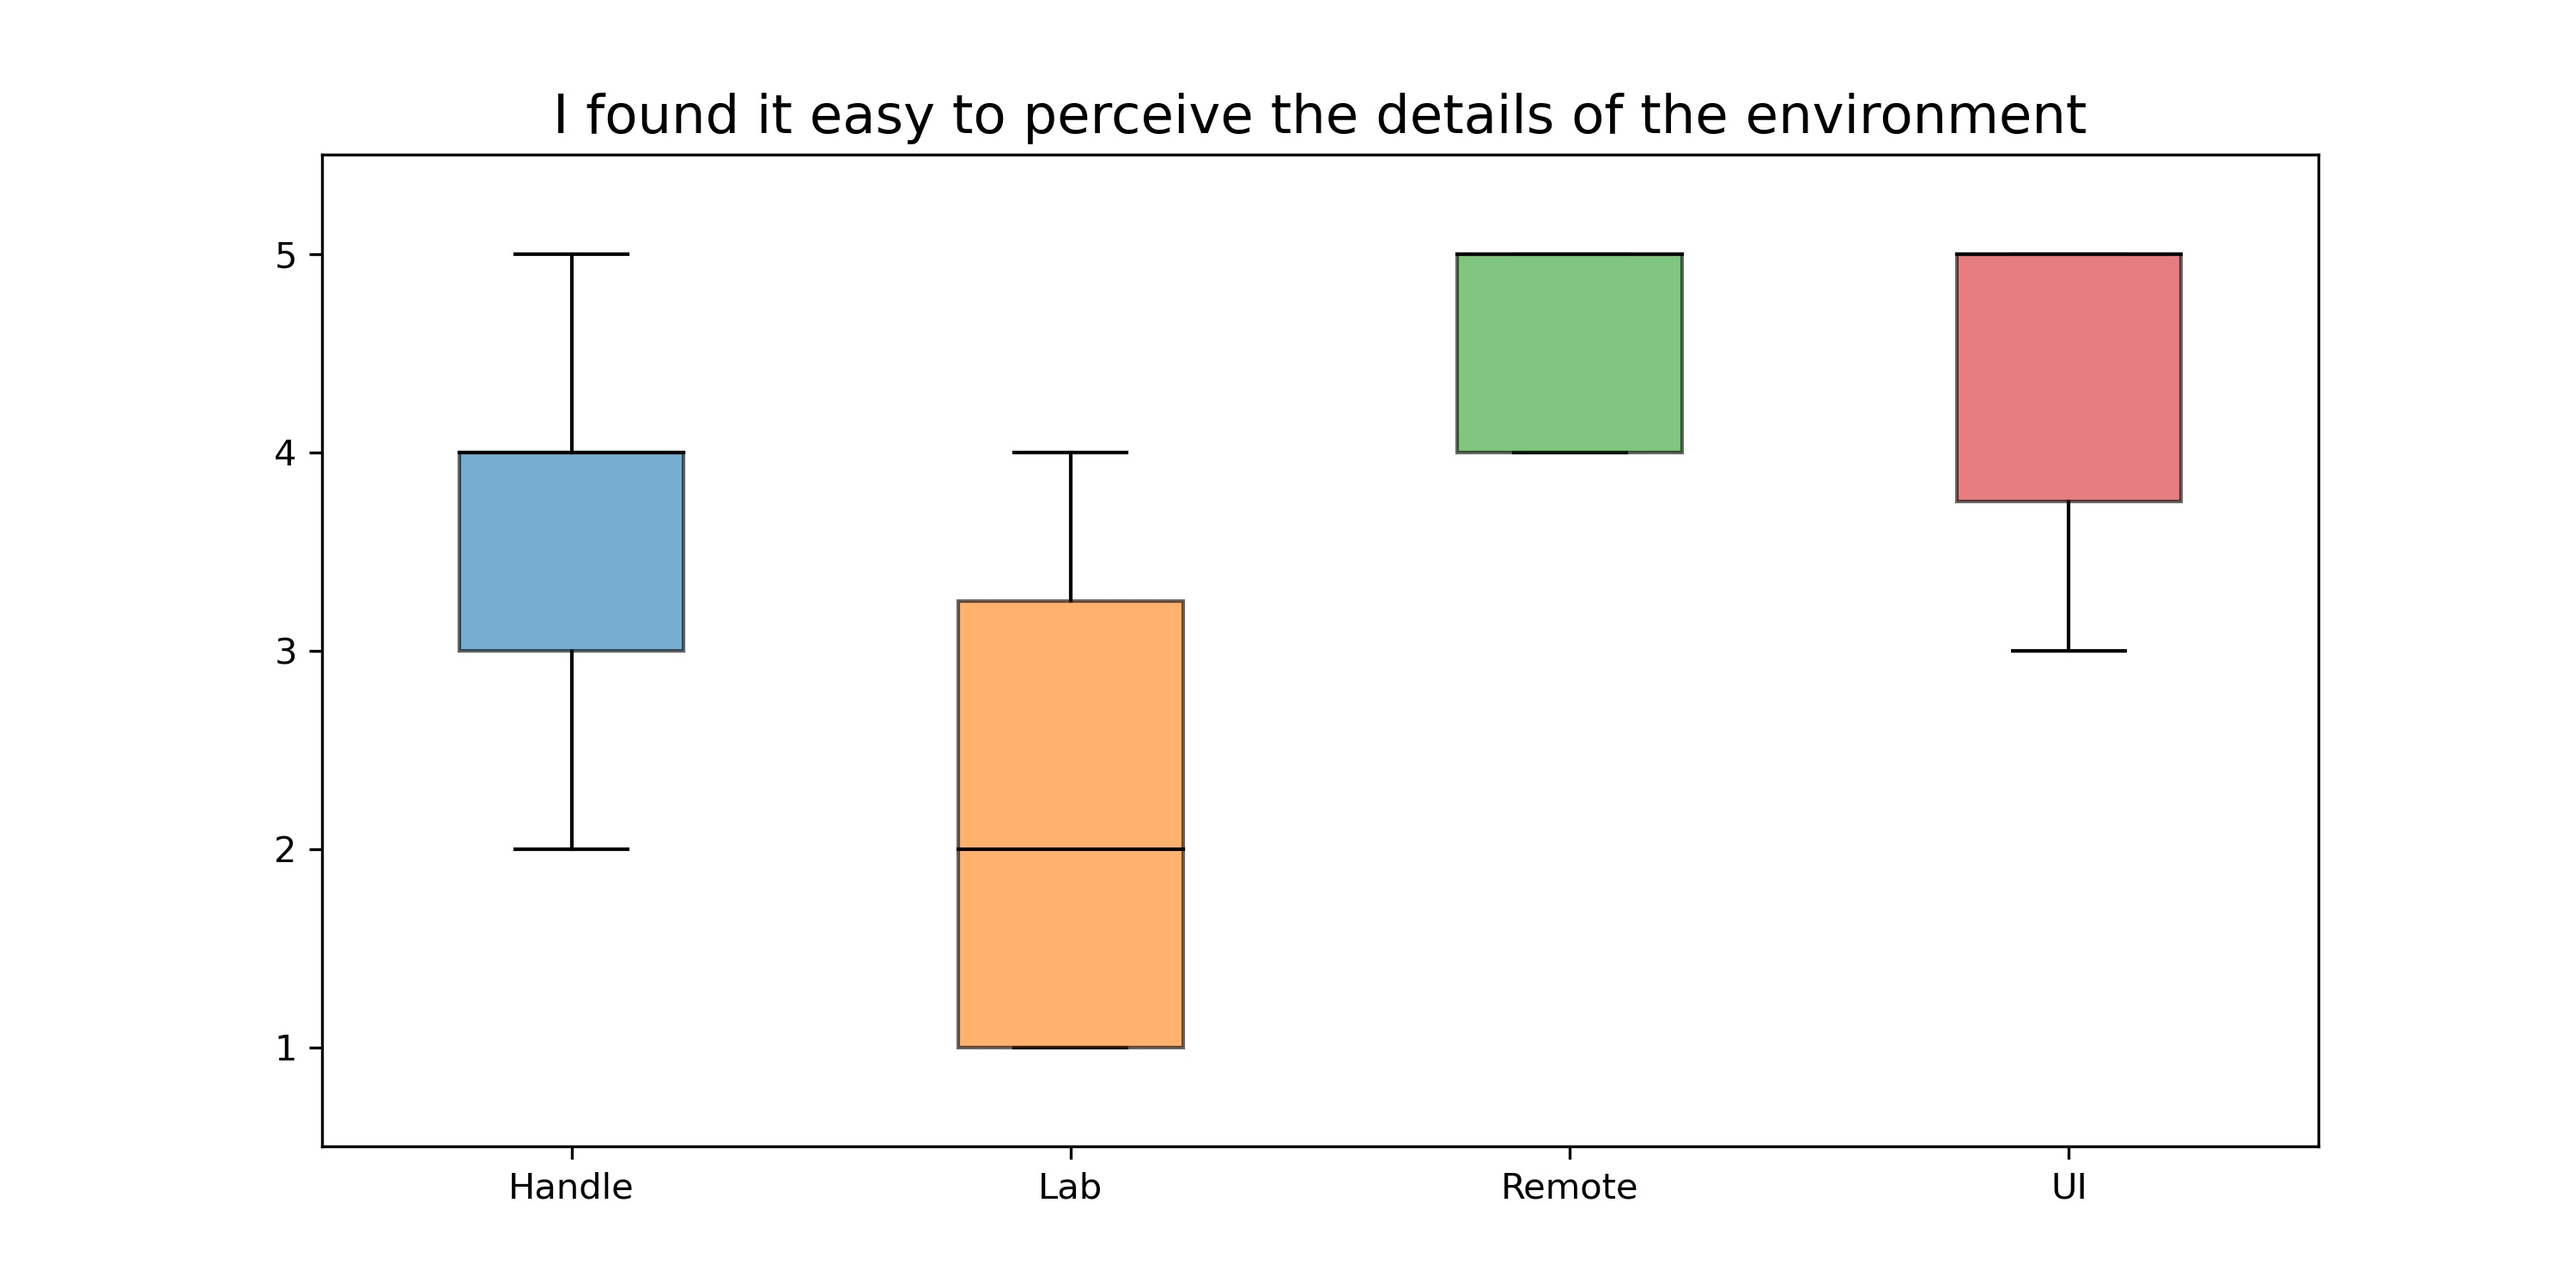
\includegraphics[height=7cm]{graphics/I found it easy to perceive the details of the environment.jpg}
    }
    \caption{Likert Questionnaire Results.(1:strongly disagree, 5:strongly agree)}
    \label{fig:liker} 
\end{figure}



\subsubsection{"I found it easy to move robot in desired position."}
The Remote Mode received a highly uniform rating. All eight participants gave it the highest score of 5. The UI Mode also showed good ratings, but two participants scored out of the majority. They explained that sometimes they forgot to cancel the follow function, causing the robot to drive to undesired locations. In this regard, Lab Mode performed the worst, with an average score of 3. And three participants gave a low score of 2 to Lab Mode.


\subsubsection{"I found it easy to concentrate on controlling the robot."}

In Handle Mode, participants seemed to have more difficulty concentrating on controlling the robot. This could be partly attributed to the fact that the participants had to adjust their distance from the robot when it was about to leave their field of view. On the other hand, participants had to control the direction and movement of the cart, which was not as easy in the Handle Mode as in the Remote and UI modes. Therefore, although participants needed to adjust their position while controlling the robot in all three modes, the other two modes scored better than Handle Mode. Some participants thought that they could concentrate well in Lab Mode because they did not need to turn their heads and adjust their positions frequently as in the other 3 modes. However, some participants held the opposite opinion. They stated that they needed to recall how the lab operated, and that multiple screens would also cause distractions.


\subsubsection{"I found it easy to perceive the details of the environment."}
The Lab Mode had the worst rating. This could partially be explained by the use of a screen to show the scene, rather than through immersion. Another reason was the poor display quality of the screen, which some participants felt was very blurred, making it impossible for them to observe the details of the scene. The results of Handle Mode differed greatly. Five participants gave a rating higher than 4. However, three participants gave a score of 2 or 3. The reasons were similar to what was mentioned in last question. The difficulty of operation and the need to alternate between controlling the robot and their own position made it difficult for them to focus on the scene.


\section{Qualitative Results}
This section will discuss the feedback from participants. Overall, every participant gave positive comments about operating the robot in a \gls{vr} platform. They thought the proposed system was exciting and did allow them to perceive more details in the post-disaster environment than the traditional video-based manipulation. The feedbacks obtained from each mode will be listed next.

70\% of participants ranked Lab Mode as the least preferred mode. Some participants were very unaccustomed to using \gls{vr} handles to grasp objects, which made it difficult for them to operate the robot with virtual joysticks smoothly. For those who have \gls{vr} experience, even without any hints and learning, they subconsciously understood what each button and joystick represented and were able to operate the robot directly. Nevertheless, for the actual rescue experience in the test focus, both kinds of participants responded that the robot's operation was more complex and difficult than the other modes. Participants attributed the reasons to obstacles in the environment. One of the participants said: "\textit{There is no physical access to the joystick. So it is slightly tough for me to control the robot.}" In some cases, when the robot was stuck in a corner, it took them much effort to get the robot out of this situation. Also, since the Lab Mode uses a simulated screen, the Lab Mode is not as good as the other three in terms of observing the details of the scene. Participants felt that the simulated screen was blurred, and the frequent switching between multiple screens made them very tired. 

%Handle
Handle Mode directly uses motion controllers for moving the robot. The evaluation of this operation mode depends in large part on the design of the motion controllers. The proposed system uses the touchpad on the \gls{htc} motion controllers to control the direction of the robot. More than half of the users thought that the touchpad made them less flexible when operating the robot's steering. Participants were often unable to accurately touch the correct position of the touchpad when using it, and it was very likely to be touched by mistake. At the end of the experiment, these participants were additionally invited to re-operate the robot using the \gls{vr} controller with thumb sticks, and said that using thumb sticks was easier for them to control the direction. Some participants said that they did not like the two monitoring screens provided by this mode. The additional surveillance screens made them subconsciously distracted to observe them, preventing them from concentrating on the rescue mission. Others, however, thought that the monitor was particularly helpful. As it was very difficult to control the robot while teleporting themselves, they first relied on the monitor screen to drive the robot to a place, and then teleported themselves to the location of the robot. The experiment also found that participants tended to forget that the two monitor screens could be closed, and they usually tried to drag the screens to places where they did not affect their view and dragged them back when they wanted to use them.

Remote Mode and UI Mode that use intelligent obstacle avoidance driving algorithm were most well-received. Participants felt that in both modes they did not need to worry about how to control the robot's steering and forward speed, but that the computer was responsible for everything, allowing them to focus on virtual world exploration.

For the UI Mode, one of the participants remarked: "\textit{I can just let the robot follow me. I don't need to think about how to operate the robot. This way I can concentrate on the rescue.}" In the user study, all participants could easily learn how to operate the UI menu. This may be explained by the fact that the menu interface was very familiar to them. It was observed that all participants did not use the direction buttons and monitoring screens in the virtual menu. At the beginning of the test, they all turned on the follow function directly and adjusted the robot's driving speed to the maximum. After that, the robot was more like a moveable \gls{lidar} sensor. This therefore led to the fact that these participants could completely disregard the location of the robot and just explore the \gls{vr} world on their own. One participant in the experiment teleported so fast that when he reached a location and had been waiting for a while, the robot was still on its way. In fact, the problem of not being able to find the robot happened in Handle Mode as well.

In contrast, Remote Mode solves this problem of the robot not being in view. One participant stated that “\textit{The robot is always in sight, so I don't have to waste extra time looking for the robot. Control of the robot is also very easy}.” Another participant reflected that after setting the destination of the trolley operation, he would subconsciously observe the movement of the robots, thus making him always know where the robot was. They also thought it was very easy in this mode to operate the robot. Many participants alternated between using the right- and left-hand rays, first setting the robot's moving target point with the right-hand ray, and then teleporting themselves there with the left-hand ray. The backup measures (remote controller) were almost not used in the actual test. When it came to the robot's inability to navigate automatically to the destination, the participants preferred to move the robot by resetting the destination point.

In addition to this, participants were found lost in each of the operation modes. They could forget whether the place was already visited by themselves. Similar behavior was observed in all participants. They passed by the same place over and over again, and sometimes simply stayed within the confines of a known scene and did not explore further.

